\documentclass[10pt]{article}
%\usepackage[french]{babel}
\usepackage{fontspec}
\usepackage{polyglossia}
\setdefaultlanguage{french}
\usepackage[a4paper,top=1cm,bottom=1cm]{geometry}
%\usepackage{url,hyperref}
%\usepackage{siunitx}
%\usepackage{schemabloc}
%\usepackage{listings}
%\usepackage{auto-pst-pdf}
%\usepackage{pst-circ}
%\usepackage{soul}
%\usepackage{verbatim}
\usepackage{lmodern}
%\usepackage{tikz}
%\usepackage[european,cuteinductors,siunitx]{circuitikz}
\usepackage{xunicode,xltxtra}
\usepackage{graphicx}
%\usepackage{amsmath}
\usepackage{minted}
%\usepackage{multicol}
\title{
\includegraphics{inp-enseeiht} \\ ~ \\ ~ \\ ~ \\ ~ \\ Exercices de Matlab \\ Seconde séance : Graphiques 2D \& 3D }
\author{Guilhem Saurel}
\date{\today}
\renewcommand{\thesubsection}{\thesection .\Alph{subsection}}
\begin{document}

 \begin{titlepage}
  \maketitle
  \tableofcontents
 \end{titlepage}

 \section{Résolution d’un système d’équation non-linéaires}
  \inputminted[linenos]{matlab}{ResolNum.m}
  \begin{center}
   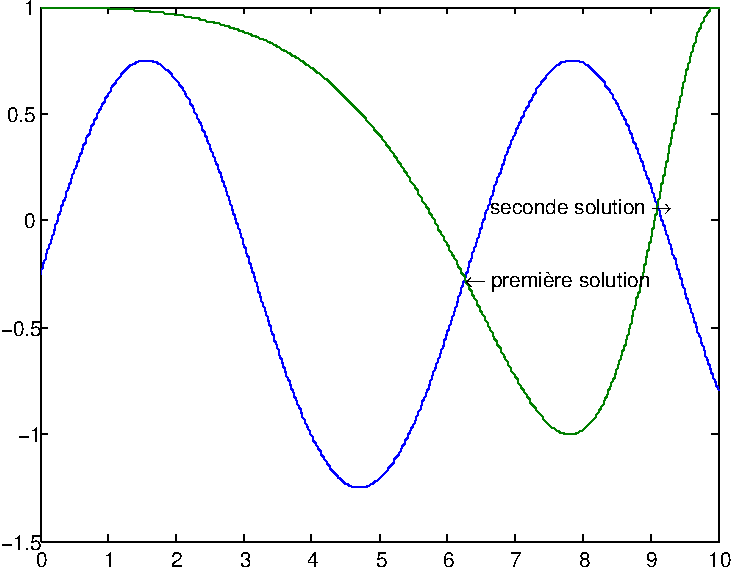
\includegraphics{ResolNum}
  \end{center}
  \newpage

 \section{Réponse d’un filtre passe-bande}
  \inputminted[linenos]{matlab}{PasseBande.m}
  \begin{center}
   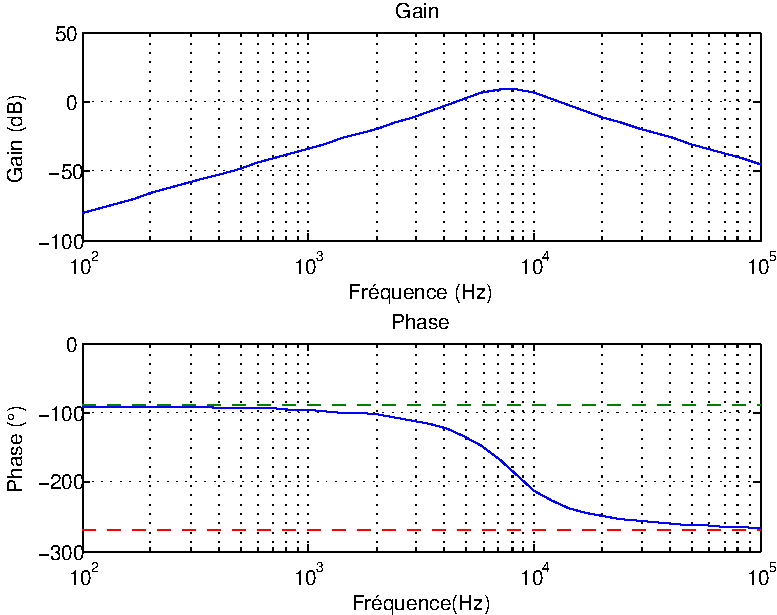
\includegraphics{PasseBande}
  \end{center}
  \newpage

 \section{Onde Stationnaire sur une ligne transmission}
  \inputminted[linenos]{matlab}{OndeStationnaire.m}
  \begin{center}
   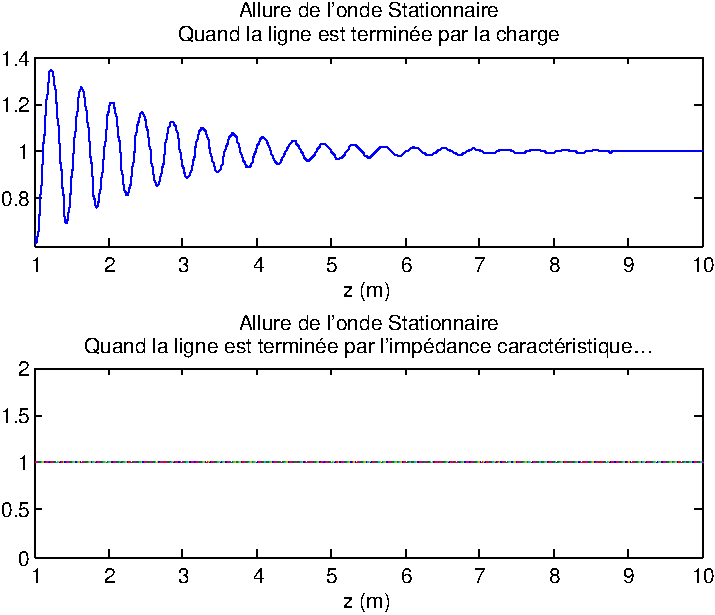
\includegraphics{OndeStationnaire}
  \end{center}
  \newpage

 \section{Tracé 3D}
  \inputminted[linenos]{matlab}{troisD.m}
  \begin{center}
   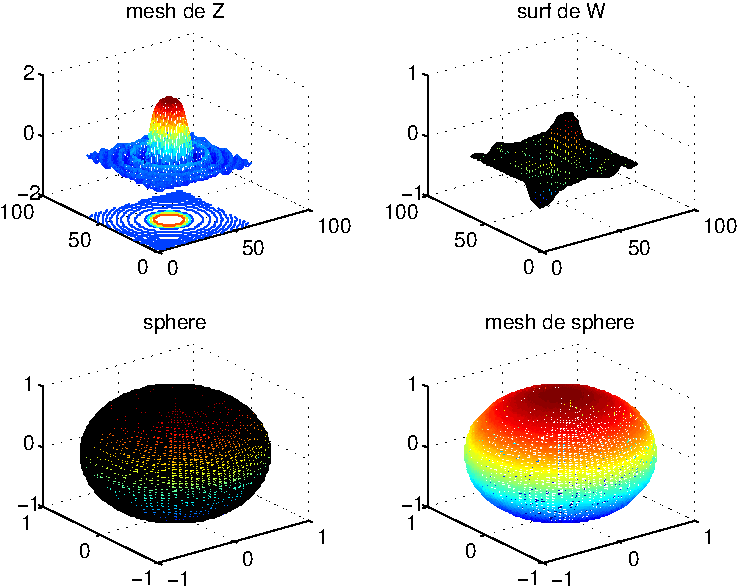
\includegraphics{TroisD}
  \end{center}
  \newpage

 \section{Modes dans un guide d’ondes}
  \inputminted[linenos]{matlab}{GuideDOndes.m}
  \begin{center}
   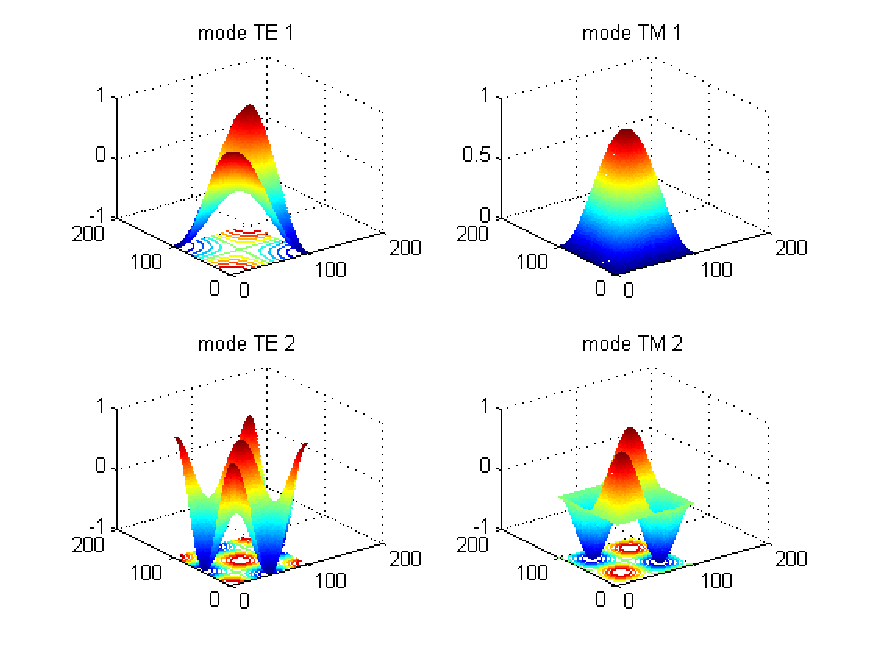
\includegraphics{GuideDOndes}
  \end{center}

\end{document}
